% !TEX root = ../main.tex

\chapter{Resolving the Multiple Withdrawal Attack on ERC20 Tokens}\label{ch:multiple}

\textit{This chapter is based on the paper ``Resolving the Multiple Withdrawal Attack on ERC-20 Tokens'' ~\cite{MultipleWithdrawal} supervised by Dr. \supv. The paper is published in the 2019 IEEE European Symposium on Security and Privacy Workshops (EuroS\&PW), at KTH Royal Institute of Technology in Stockholm, Sweden.}

\section{Introduction}
In this chapter, we present a summary of our research on smart contracts and their subset, ERC-20 tokens. First, we examine the \mwa in ERC-20 tokens, which was identified in November 2016 and has remained unresolved without a reliable solution. We then review ten proposed solutions and present two proposals to address this issue. By implementing one of the proposals, the security of future ERC-20 smart contracts will be significantly improved.

Since the introduction of ERC-20 in November 2015, several vulnerabilities have been discovered. In November 2016, a security issue called \mwa was opened on GitHub~\cite{AttackVector,Resolution}. The attack originates from two methods in the ERC-20 standard for approving and transferring tokens. The use of these functions in an adverse environment (\eg front-running~\cite{eskandari2019sok}) could result in more tokens being spent than what was intended. This issue is still open and several solutions have been made to mitigate it.

\begin{figure}[t]
	\centering
	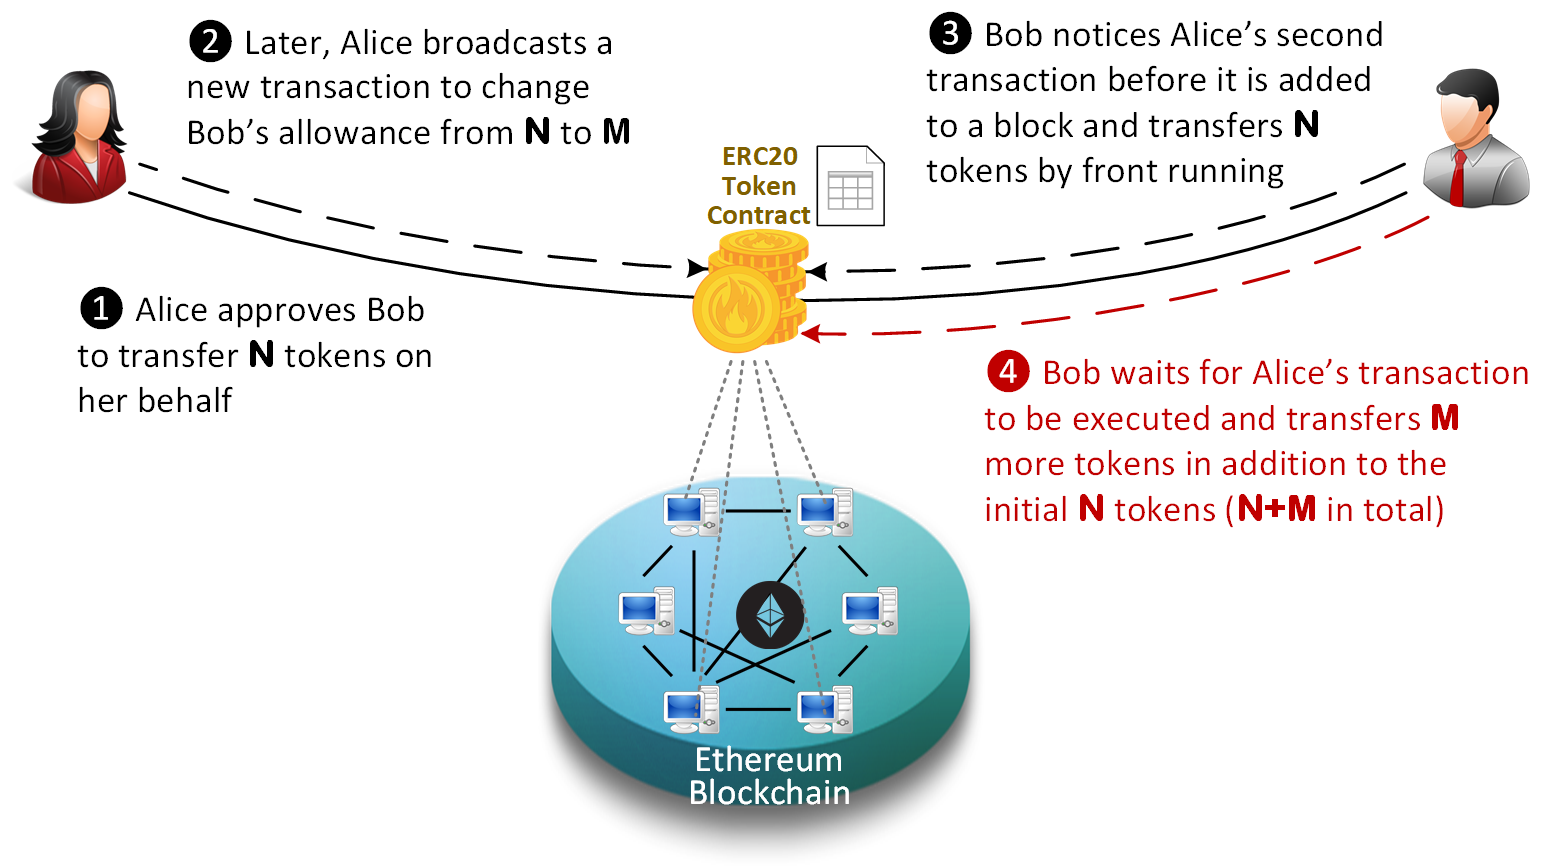
\includegraphics[width=\textwidth,keepaspectratio]{multiple_withdrawal.png}
	\caption[Steps for the \mwa in ERC-20 tokens]{Steps to perform the \mwa in ERC-20 tokens.}
	\label{fig:mwa}
\end{figure}

According to the ERC-20 API definition, the \texttt{approve} function allows a spender (\eg user, wallet or other smart contracts) to withdraw up to an allowed amount of tokens from token pool of the approver. If this function is called again, it overwrites the current allowance with the new input value. On the other hand, the \texttt{transferFrom} function allows the spender to actually transfer tokens from the approver to anyone they choose (importantly: not necessarily themselves). The contract updates balance of transaction parties accordingly. An adversary can exploit the gap between the confirmation of the \texttt{approve} and \texttt{transferFrom} functions since the \texttt{approve} method replaces the current spender allowance with the new amount, regardless of whether the spender already transferred any tokens or not. This functionality of the \texttt{approve} method is shaped by the language of the standard and cannot be changed. Furthermore, while variables change and events are logged, this information is ambiguous and cannot fully distinguish between possible traces. Consider steps in Figure \ref{fig:mwa}:

\begin{enumerate}
	\item Alice allows Bob to transfer N tokens on her behalf by \texttt{approve(\_Bob, N)}.
	\item Later, Alice changes Bob's approval from N to M by \texttt{approve(\_Bob, M)}.
	\item Bob notices Alice's second transaction after its broadcast to the Ethereum network but before adding to a block.
	\item Bob front-runs (using an asymmetric insertion attack~\cite{eskandari2019sok}) the original transaction with a call to \texttt{transferFrom(\_Alice, \_Bob, N)}. If a miner is incentivized (\eg by Bob offering high gas) to add this transaction before Alice's, it will transfer N of Alice's tokens to Bob.
	\item Alice's transaction will then be executed which changes Bob's approval to M.
	\item Bob can call \texttt{transferFrom} method again and transfer M additional tokens.
\end{enumerate}
In summary, in attempting to change Bob's allowance from N to M, Alice makes it possible for Bob to transfer N+M of her tokens. We operate on the assumption that a secure implementation would prevent Bob from withdrawing Alice's tokens multiple times when the allowance changes from N to M. A proposed solution should prevent this from happening by allowing only M approved tokens to be transferred after changing from the initial N tokens.

\section{Significance of Mitigation}
ERC-20 tokens are important component of Ethereum's supplementary financial system that have many financial (as well as non-financial) uses and could hold considerable value (potentially exceeding the value of Ether itself). There has been more than 64,000 functional ERC-20 tokens as of early 2019~\cite{victormeasuring} that might be vulnerable to this attack. Furthermore, ERC-20 tokens that have already been issued cannot easily migrate to a new secure implementation and should these tokens appreciate in value in the future. Resolving the attack also serves as basis for other extended standards, such as ERC-777~\cite{EIP777} to be backward compatible with ERC-20 interface~\cite{frowis2018detecting}. Finally, firms that hold ERC-20 tokens require assurance of their security, particularly in the case that they require their financial statements to be audited---an issue like this could lead to further hesitation by auditors.

\section{Transaction-Ordering Dependence}
The \mwa could happen when multiple transactions invoke the same contract at roughly the same time. The next block will most likely execute and include these transactions. For example, considering contract $c$ at state $s_0$, a miner may receive transactions $T_i$ and $T_j$ from two different users ($|T_i-T_j| \leq 12 \; seconds$). Depending on the miner decision on the order of $T_i$, $T_j$, there would be uncertainty about the invocation results (\ie $s_0 \xrightarrow{T_i} s_1 \xrightarrow{T_j} s_2$ or $s_0 \xrightarrow{T_j} s_3 \xrightarrow{T_i} s_4$). Thus, there might be a discrepancy between the state of the contract when users invoke the transaction and the actual state when the execution happens \cite{SmartContractSecurity}. This issue might happen in one of the following scenarios:
\begin{itemize}
	\item \textbf{Race-condition:} A non-malicious scenario wherein two users (or contracts) attempt to perform two invocations at the same time. Concurrent transactions may lead to an unexpected results due to uncertainty in the execution order. For example, in a decentralized exchange, sellers might update ask prices while buyers submit the bid prices based on the observed ask prices. Depending on the transaction ordering, buy requests may or may not go through, or buyers may pay more for a dropped price.
	
	\item \textbf{Front-running:} A malicious scenario wherein miners can change sequence of new transactions to gain profit. This is the required condition to perform \mwa in ERC-20 tokens where Alice attempts to change Bob’s allowance from N to M, but she made it possible for Bob (who is running a mining node) to transfer N+M due to change in the execution order of \texttt{approve()} and \texttt{transferFrom()} transactions.
\end{itemize}
Mitigating this vulnerability is not easy and depends on the logic of the smart contract. It can happen since there is a time gap around 12 seconds between (1) broadcasting the transaction and (2) including the transaction in a new block. Thus, a malicious miner can listen to the network and change transaction orders for financial advantages. This is part of Ethereum's consensus protocol that allows arbitrary miners to participate in the network. The consensus protocol elects a leader among all miners and the leader then broadcasts its proposed block to all nodes. After block validation, all nodes update their local copy to include the new block.

There are a few logical places to address this attack. Ideally the token author (instead of the token holders) would mitigate the attack within the ERC-20 smart contract. Since two methods are involved in the attack, it could be addressed within the \texttt{approve} and/or \texttt{transferFrom} method. By contrast, token owners have no control over the implementation of the contract and are relegated to mitigate the attack by monitoring the contract around the time allowance changes are made. Since this is very difficult, we concentrate on mitigating the attack in the contract itself.

\section{Evaluating Proposed Mitigations}
The authors of the ERC-20~\cite{Interface} reference two sample implementations from OpenZeppelin~\cite{OpenZeppelin_Token} and ConsenSys~\cite{ConsenSys_Token}. OpenZeppelin implementation mitigates the attack by introducing two additional methods to increase or decrease approved tokens, and the ConsenSys code does not attempt to resolve it. Additional implementations have a variety of different trade-offs in mitigating the issue. We evaluate ten proposed solutions and develop a set of criteria that encompass backwards compatibility, interoperability, adherence to the ERC-20 standard, and attack mitigation. 

The summary of evaluations along with our two proposals is provided in Figure \ref{fig:mitigations}. Proposal 1 mitigates the attack by comparing transferred tokens with new allowance. It is not fully compliant with ERC-20 specifications since the allowance result does not always match what is requested. In proposal 2, a new variable is defined to keep track of transferred tokens and prevents transfers in the case of already transferred tokens. We examine the details of the two proposals in Sections \ref{subsec:prop1} and \ref{subsec:prop2}.

\begin{figure}[t]
	\centering
	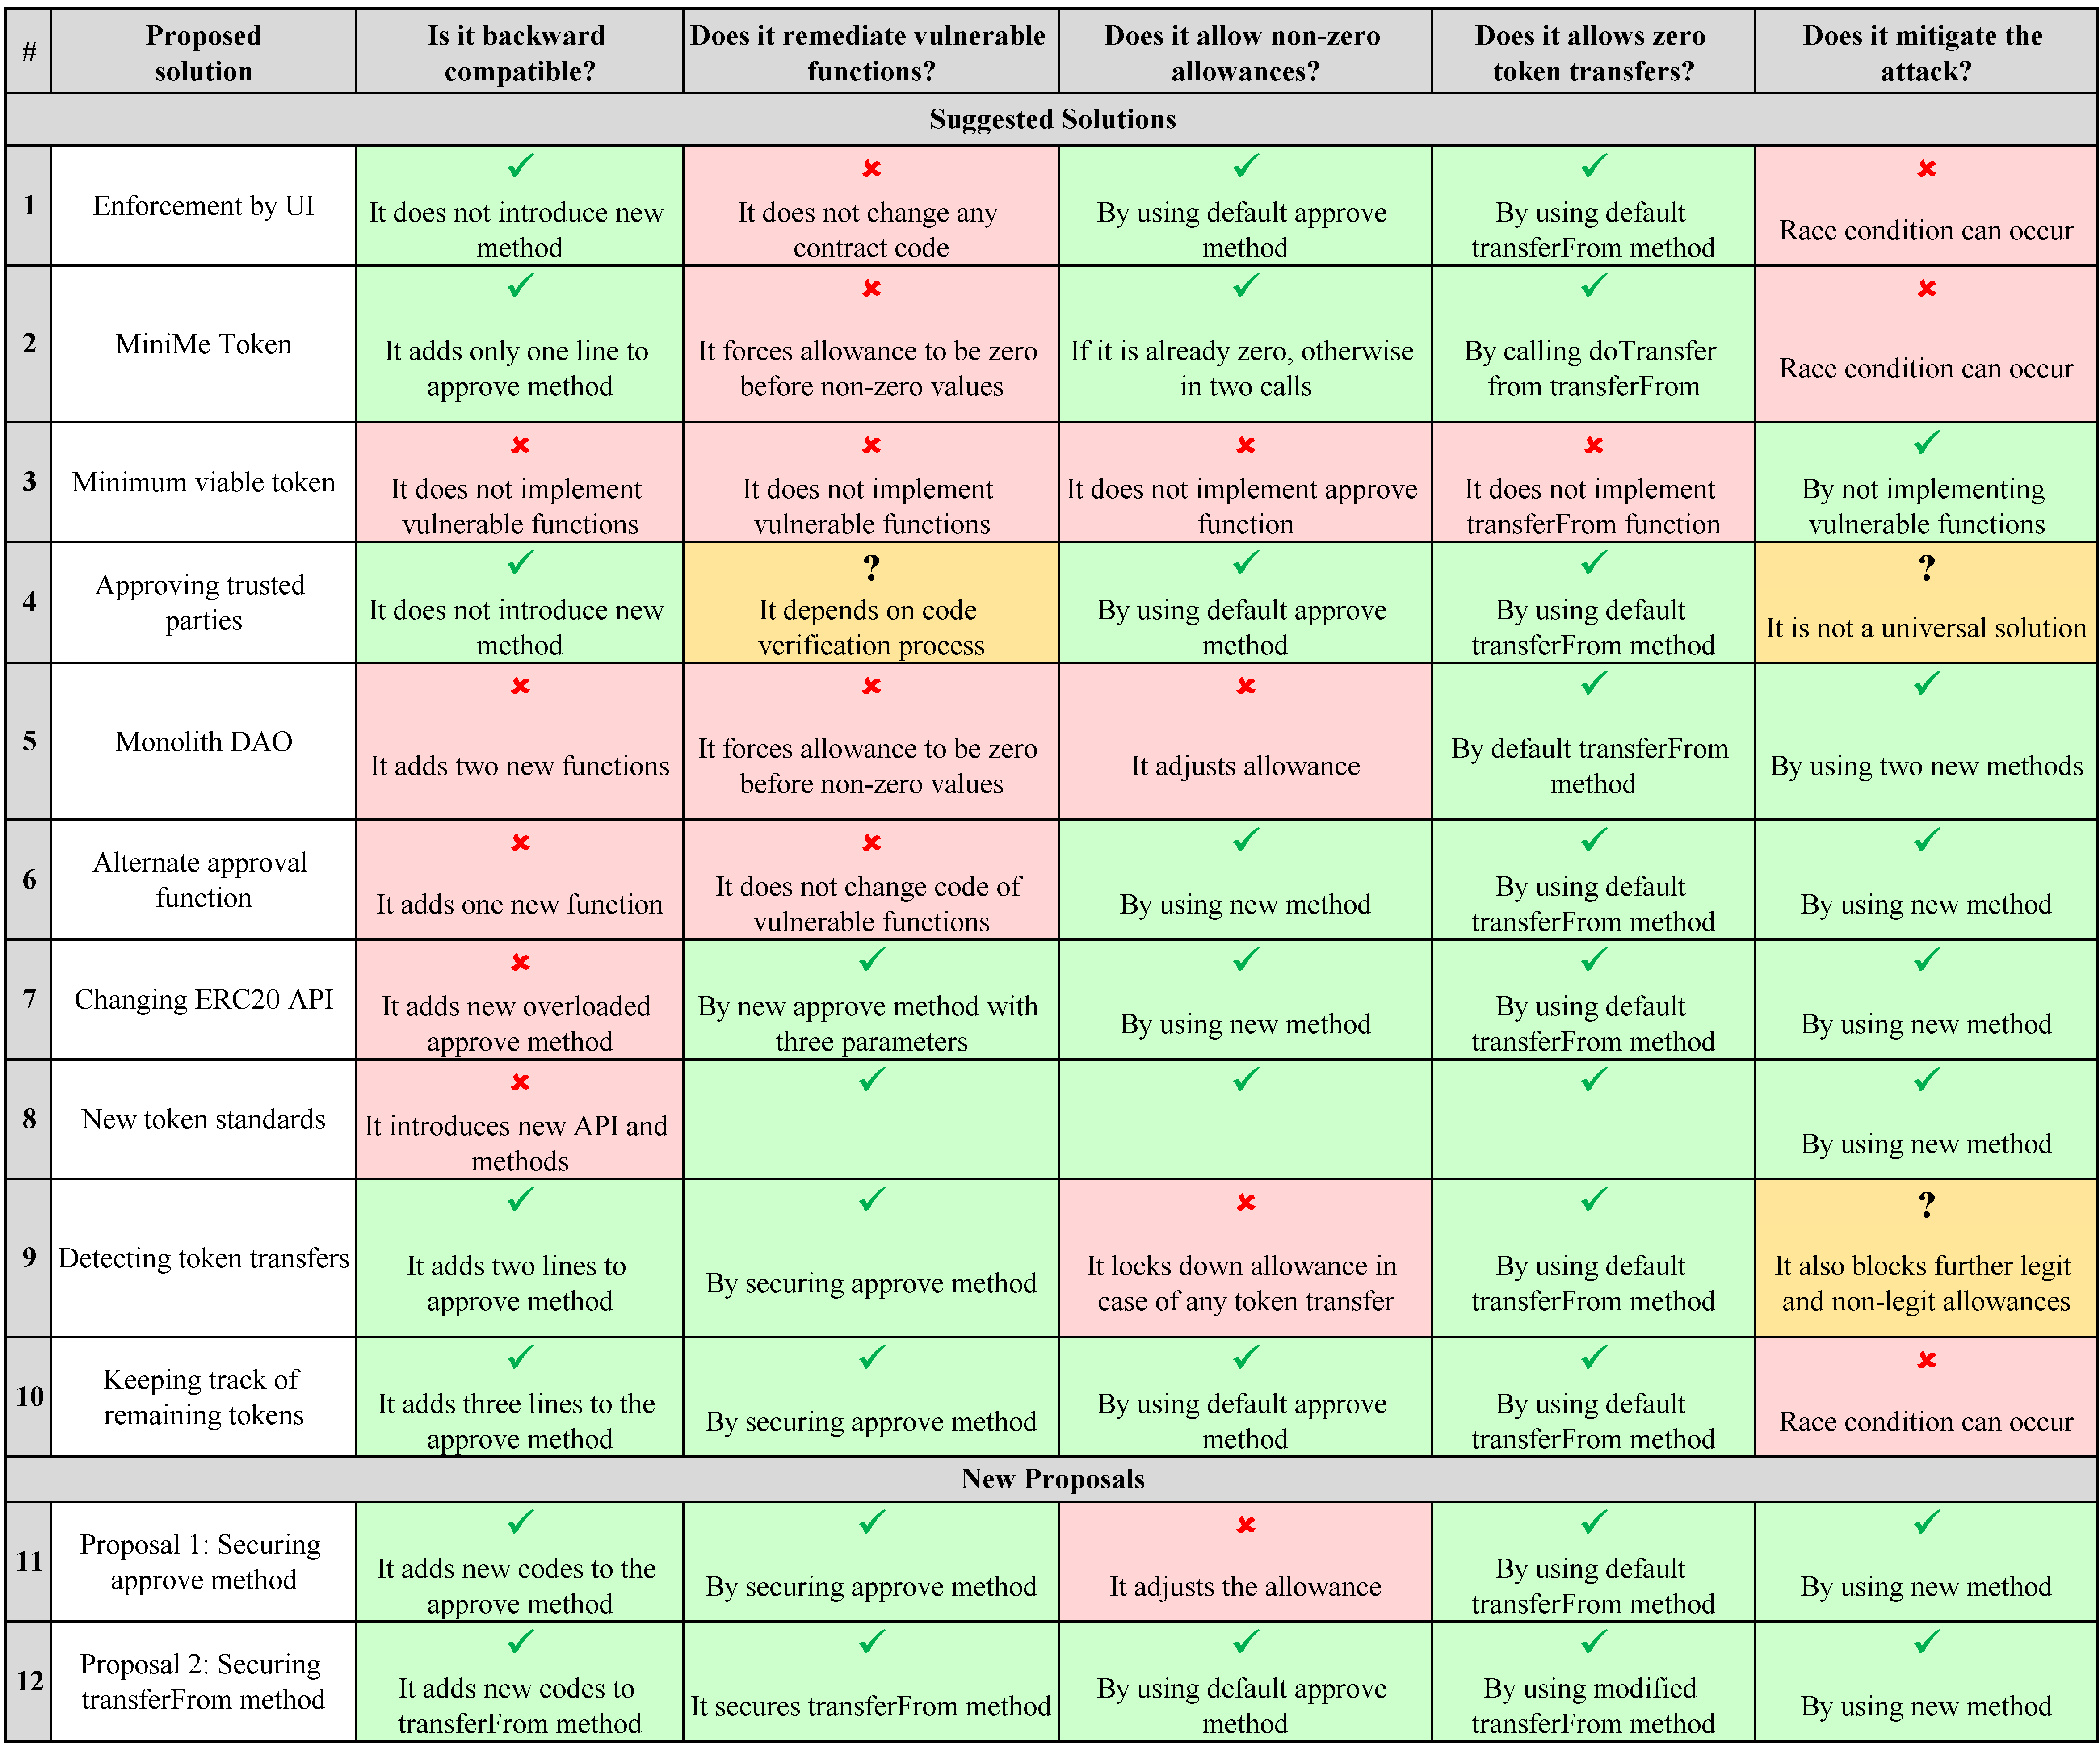
\includegraphics[width=\textwidth,keepaspectratio]{evaluation_table.png}
	\caption[Evaluation of ten \mwa mitigation proposals]{Evaluation of the ten proposed mitigations for the \mwa.}
	\label{fig:mitigations}
\end{figure}

\section{New Mitigations}
Since no mitigation is fully satisfactory, we develop two additional solutions based on the \textit{Compare and Set (CAS)} pattern~\cite{CompareSwap}. We study in detail possible implementations of the \texttt{approve} and \texttt{transferFrom} methods. We argue that a CAS-based approach can never adequately deploy a secure \texttt{approve} method while adhering to the ERC-20 standard. We therefore prioritize adherence to the ERC-20 standard. While deviating from the standard might become acceptable if there is no possible way to conform with it and maintain security, we consider that a last resort. Indeed, as we will show, it is possible to secure an ERC-20 contract within the constraints of the standard~\cite{Interface}. Requirements of an ideal solution are summarized here:
\begin{itemize}
	\item The input to \texttt{approve} method is a new allowance and not a relative adjustment.
	\item The result of \texttt{approve} method will overwrite the current allowance with the new allowance.
	\item A call to \texttt{transferFrom} on an input of 0 tokens will execute as a normal transfer and emit a \texttt{Transfer} event.
	\item A spender can call \texttt{transferFrom} multiple times up to the allowed amount.
	\item Transferring up to any initial allowance is always a legitimate transfer.
	\item An ideal solution cannot rely on overloading existing methods or introducing new methods outside of ERC-20, as existing DApps and web apps would have to be modified to interoperate. A solution must eliminate all race conditions.
\end{itemize}
We now propose two solutions that that mitigates the attack by: (i) securing implementation of the \texttt{approve} method, (ii) securing implementation of the \texttt{transferFrom}.

\subsection{Proposal 1: Securing Implementation of \texttt{approve}}\label{subsec:prop1}
By implementing the CAS pattern~\cite{CompareSwap} in the \texttt{approve} method (highlighted code in the code snippet of Figure \ref{fig:approve}), we set up a small state machine so that new allowances can be set atomically after a comparison with transferred tokens. This tracking also requires adding a new variable to the \texttt{transferFrom} method. Since this is an internal variable, it is not visible to already deployed smart and keeps the \texttt{transferFrom} function compatible. Similarly, a block of code is added to the \texttt{approve} function (Shown with a red box in the code snippet of Figure \ref{fig:approve}) to work in both cases with zero and non-zero allowances. This new logic in the \texttt{approve} function compares a new allowance---passed as \texttt{\_tokens} argument to the function---with the current allowance of the spender and the already transferred tokens.

\begin{figure}[t]
	\centering
	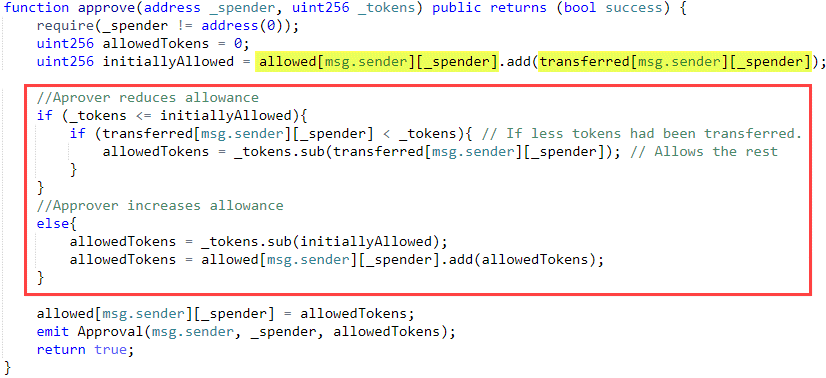
\includegraphics[width=\textwidth,keepaspectratio]{approve.png}
	\caption[Resolving \mwa in \texttt{approve}]{Resolving \mwa by implementing the CAS pattern in the \texttt{approve} method.}
	\label{fig:approve}
\end{figure}

Allowance are saved in \texttt{allowed[msg.sender][\_spender]} variable as in typical ERC-20 implementation, and \texttt{transferred[msg.sender][\_spender]} is the new state. The method decides to increase or decrease the current allowance based on this comparison. If the new allowance is less than initial allowance---sum of \texttt{allowance} and \texttt{transferred} variables---it denotes decreasing of allowance, otherwise increasing of allowance is intended. Such a modified \texttt{approve} function prevents the attack by either increasing or decreasing the allowance instead of setting it to an explicit value. 

In summary, we can use the CAS\anote{cas} pattern to implement a secure \texttt{approve} method that can mitigate the attack effectively. However, it violates one of the ERC-20 specifications that says: ``If \texttt{approve} function is called again, it overwrites the current allowance with \texttt{\_value}". Our solution does not comply with this as the resulting allowance can be different than what is passed by the approver. Furthermore we argue that is in fact impossible to secure the \texttt{approve} method without adjusting the allowance. Therefore the \texttt{approve} method has to adjust the allowance according to transferred tokens, not based on passed input values to the \texttt{approve} method. Overall, there seems to be no solution to secure the \texttt{approve} method while adhering specification of ERC-20 standard. In proposal 2, the focus is to take this requirement into consideration by securing the \texttt{transferFrom} method.

\subsection{Proposal 2: Securing Implementation of \texttt{transferFrom}}\label{subsec:prop2}
As an alternative to Proposal 1, we can also consider securing the \texttt{transferFrom} method. As specified by the ERC-20 standard, the goal here is to prevent the spender from transferring more tokens than allowed. Based on this assumption, we should not rely solely on the allowance value in deciding whether to allow or prevent an approve and should also consider the number of transferred tokens, which requires new state as in Proposal 1. Our solution, which is compliant with a careful reading of ERC-20 specifications, is to interpret allowance as a `global' or `lifetime' allowance value, instead of the amount allowed at the specific time of invocation (see red boxes in the code snippet of Figure \ref{fig:transfer}). 

\begin{figure}[t]
	\centering
	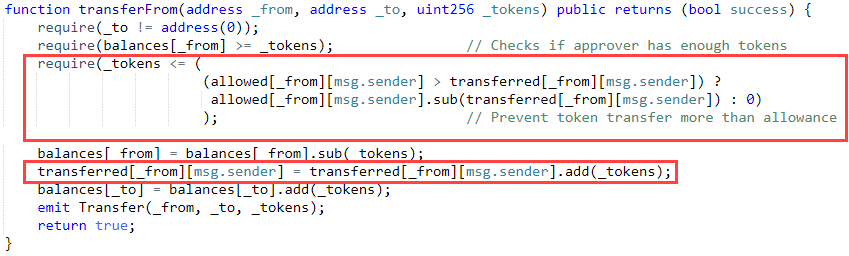
\includegraphics[width=\textwidth,keepaspectratio]{transferFrom.png}
	\caption[Resolving \mwa in \texttt{transferFrom}]{Resolving \mwa by securing the \texttt{transferFrom}.}
	\label{fig:transfer}
\end{figure}

\begin{example}
	Alice approves Bob for 50 tokens, Bob transfers 50 tokens, Alice approves Bob for 30 (more) tokens, and Bob transfers 30 tokens. In our implementation, Alice would approve Bob for 50 tokens and he transfers 50 tokens. To approve Bob for 30 more tokens, she approves Bob for 80 tokens. He has already spent 50 of these 80 tokens so he will only be allowed to transfer an addition 30. Thus 80 is his lifetime allowance and 50 (kept internally) is the amount he has transferred. 
\end{example}

In a bit more detail, consider the following, which prevents multiple withdrawals by modifying the implementation of \texttt{transferFrom} but keeping \texttt{approve} untouched:
\begin{enumerate}
	\item Alice approves Bob to transfer 100 tokens
	\item Alice broadcasts an approval of 70, decreasing Bob's allowance.
	\item Bob front-runs Alice’s transaction and transfers 100 tokens (remark: a legitimate transfer).
	\item Alice's transaction is confirmed and sets Bob allowance to 70 by the default \texttt{approve} method.
	\item Bob's noticed the new allowance and tries to move 70 additional tokens by broadcasting \texttt{transferFrom(\_Bob,70)}. 
	\item Since Bob has already transferred more than 70 tokens, his transaction fails and prevents multiple withdrawal. 
	\item After all, Bob’s allowance is set at 70 and his transferred tokens are set at 100.
\end{enumerate}

Our advice to developers is to use proposal 2 which is compatible with the ERC-20 token standard. Additionally, while this is a deep dive into a specific issue with ERC-20, it also illustrates a number of higher level lessons for blockchain developers. When ERC-20 standard was first implemented, it changed how people used Ethereum, giving rise to an ICO craze with its ease of use~\cite{fenu2018ico}. This led to the deployment of thousands of early implementation of ERC-20 tokens which has resulted in numerous attacks on different implementations. Now we see decentralized exchanges relying on existing ERC-20 tokens and the \mwa seems too important to ignore. Fixing existing ERC-20 code will help future deployments but cannot fix the already deployed tokens. In addition to deploying secure contracts, we suggest blockchain developers conduct external audits and consider security-by-design practices when dealing with other smart contract implementations.

\subsubsection{Performance} In order to evaluate functionality of the new \texttt{approve} and \texttt{transferFrom} functions, we have implemented a standard ERC-20 token (TKNv1\anote{impl1}) along side the proposed ERC-20 token (TKNv2\anote{impl2}). Our testing for different input values shows that TKNv2 can address the \mwa by making front-running gains ineffective. Moreover, we compared these two tokens in term of gas consumption. The \texttt{approve} function in TKNv2 uses almost the same amount of gas as TKNv1, however, gas consumption of \texttt{transferFrom} in TKNv2 is around 37\% more than TKNv1. This difference in TKNv2 is because of maintaining a new mapping variable for tracking transferred tokens. In term of compatibility, both are equivalent interoperable with standard wallets (\eg MetaMask and MEV) and have not raised any transfer issues. We believe this is acceptable for having a secure ERC20 token.

\section{Contributions}
We evaluate ten proposed mitigations for the \mwa and develop a set of criteria that encompass backwards compatibility, interoperability, adherence to the ERC-20 standard, and attack mitigation. Since no mitigation is fully satisfactory, we develop two additional solutions based on the \textit{Compare and Set (CAS)} pattern. We study in detail possible implementations of ERC-20's \texttt{approve} and \texttt{transferFrom} methods. We argue that a CAS-based approach can never adequately deploy a secure \texttt{approve} method while adhering to the ERC-20 standard. We then propose a secure implementation of the \texttt{transferFrom} method that mitigates the attack and fully satisfies the ERC-20 standard. It consumes 37\% more gas compared with the non-secure \texttt{transferFrom} method, which appears to be acceptable for achieving a secure ERC-20 implementation that protects user investments and provide a secure token transfer mechanism.

\section{Discussion}
This chapter was a deep dive into a specific issue with ERC-20, illustrating a number of higher level lessons for blockchain developers. When ERC-20 standard was first implemented, it changed how people used Ethereum, giving rise to an ICO craze with its ease of use~\cite{fenu2018ico}. This led to the deployment of thousands of early implementation of ERC-20 tokens which has resulted in numerous attacks on different implementations. Now we see decentralized exchanges relying on existing ERC-20 tokens and the \mwa seems too important to ignore. Fixing existing ERC-20 code will help future deployments but cannot fix the already deployed tokens. In addition to deploying secure contracts, we suggest blockchain developers conduct external audits and consider security-by-design practices when dealing with other smart contract implementations.